\documentclass[twoside]{article}

\usepackage[sc]{mathpazo} 
\usepackage[spanish, es-tabla]{babel}
\decimalpoint
\usepackage[utf8]{inputenc}

\usepackage[hmarginratio=1:1,top=32mm,columnsep=20pt]{geometry} % Document margins
\usepackage{multicol} % Used for the two-column layout of the document
\usepackage[hang, small,labelfont=bf,up,textfont=it,up]{caption} % Custom captions under/above floats in tables or figures
\usepackage{mathtools}
\usepackage{float} % Required for tables and figures in the multi-column environment - [H] needed
\usepackage{hyperref} % For hyperlinks in the PDF with labels

\usepackage{graphicx}
\usepackage{subcaption}
\usepackage{caption}
\graphicspath{{../python-src/Graficas/}}

\usepackage{abstract} % Allows abstract customization
\renewcommand{\abstractnamefont}{\normalfont\bfseries} % Set the "Abstract" text to bold
\renewcommand{\abstracttextfont}{\normalfont\small\itshape} % Set the abstract itself to small italic text

\usepackage{titlesec} % Allows customization of titles

\titleformat{\section}[block]{\large\scshape\centering}{\thesection.}{1em}{} % Change the look of the section titles
\titleformat{\subsection}[block]{\large\centering}{\thesubsection.}{1em}{} % Change the look of the section titles

\usepackage{fancyhdr} % Headers and footers
\pagestyle{fancy} % All pages have headers and footers
\fancyhead{} % Blank out the default header
\fancyfoot{} % Blank out the default footer
\fancyhead[C]{Calculadora Cosmológica% based on TRACS 
\hspace{4pt} $\bullet$ \hspace{4pt} Febrero 2019 } % Custom header text
\fancyfoot[RO,LE]{\thepage} % Custom footer text

\usepackage{color}
\definecolor{gray97}{gray}{.97}
\definecolor{gray75}{gray}{.75}
\definecolor{gray45}{gray}{.45}

\usepackage{listings}
\lstset{ frame=Ltb,
framerule=0pt,
aboveskip=0.5cm,
framextopmargin=3pt,
framexbottommargin=3pt,
framexleftmargin=0.4cm,
framesep=0pt,
rulesep=.4pt,
backgroundcolor=\color{gray97},
rulesepcolor=\color{black},
%
stringstyle=\ttfamily,
showstringspaces = false,
basicstyle=\small\ttfamily,
commentstyle=\color{gray45},
keywordstyle=\bfseries,
%
numbers=left,
numbersep=15pt,
numberstyle=\tiny,
numberfirstline = false,
breaklines=true,
}

% minimizar fragmentado de listados
\lstnewenvironment{listing}[1][]
{\lstset{#1}\pagebreak[0]}{\pagebreak[0]}

\lstdefinestyle{consola}
{basicstyle=\scriptsize\bf\ttfamily,
backgroundcolor=\color{gray75},
}

\lstdefinestyle{python}
{language=python,
}

%----------------------------------------------------------------------------
%	   TITLE SECTION
%----------------------------------------------------------------------------

\title{
	\vspace{-15mm}
	\fontsize{28pt}{10pt}
	\selectfont\textbf{Calculadora Cosmológica}% Article title
}

\author{
	\large
	\textsc{Jaime D\'iez Gonz\'alez-Pardo}\\[4mm]
	\fontsize{28pt}{10pt} Universidad de Cantabria \\ % Your institution
	%\thanks{A thank you or further information}\\[2mm] % Your name
	\normalsize Astrofísica \\ 
	%\normalsize{Compañeros:} \textsc{NOMBRE COMPANEROS }\\%\normalsize \href{mailto:john@smith.com}{john@smith.com} % Your email address
	%\vspace{5mm}
}

\date{ \today }


%----------------------------------------------------------------------------
%      · DOCUMENT
%----------------------------------------------------------------------------

\begin{document}


	\maketitle % Insert title


	\thispagestyle{fancy} % All pages have headers and footers

%----------------------------------------------------------------------------
%	  ABSTRACT
%----------------------------------------------------------------------------

	\begin{abstract}

		\noindent% Dummy abstract text

			Se han resuelto las ecuaciones de Friedmann para diferentes universos determinados por los parámetros cosmológicos. Para ello se desarrollado un software escrito en lenguaje Python que ha permitido resolver las ecuaciones de Friedmann utilizando métodos numéricos. Los universos han sido caracterizados por las constantes $\Omega_M$, $\Omega_R$, $\Omega_\Lambda$, $\Omega_K$ y $H_0$ tomando universos dominados por Materia, Radiación y energía oscura $\Lambda$ y analizando un universo con los parámetros actuales. El código de Python ha permitido obtener las distancias diámetro angulas $D_A$ y de luminosidad $D_L$, el factor de escala $a(t)$, el parámetro de Hubble $H(t)$, el horizonte de partículas, el radio de Hubble y la edad del universo para los cuatro universos de estudio.

	\end{abstract}

%----------------------------------------------------------------------------
%	  ARTICLE CONTENTS
%----------------------------------------------------------------------------

	%\begin{multicols}{2} % Two-column layout throughout the main article text

		\section{Introducción} % Scope of the project = rad effects + minimization
							 
			Las ecuaciónes de Friedman y de continuidad describen la dinámica de expansión del universo basándose en el principio cosmológico. Dicho principio establece que el universo a gran escala es homogéneo y isótropo. Dichas ecuaciones tratan el universo como un fluido con densidad de materia y energía $\rho$ y presión $p$.

				%H2
				\begin{equation}
					H^2(t) = \left(\frac{\dot{a}}{a} \right)^2 = \frac{8 \pi G \rho} {3} + \frac{\Lambda c^2}{3} - \frac{kc^2}{a}
					\label{eq:H2}
				\end{equation}

				%addot
				\begin{equation}
					\frac{\ddot{a}}{a} = - \frac{4\pi G}{3} \left(\rho+\frac{3p}{c^2}\right) + \frac{\Lambda c^2}{3}
					\label{eq:addot}
				\end{equation}

			En dichas ecuaciones, $H(t)$ hace referencia al parámetro de Hubble, $a(t)$ es el factor de escala de la expansión, $\Lambda$ es la constante cosmológica y $k$ la curvatura del espacio-tiempo.

			La densidad de materia y energía $\rho$ puede ser diferenciada según los constituyentes del universo. Estas densidades suelen ser expresadas en función de lós parámetros de densidad pudiendose diferenciar entre los parámetros de densidad de la materia $\Omega_{M}$, radiación $\Omega_{R}$, energía oscura $\Omega_{\Lambda}$ o curvatura $\Omega_{k}$. Cumpliendose siempre que su suma ha de valer $1$.

				% densYOmg
				\begin{equation}
					\begin{matrix}
						\rho_i = \frac{3H_0^2}{8\pi G} \Omega_i & \textrm{ con } & i = \{\textrm{M, R, } \Lambda \textrm{, }K\}
					\end{matrix}
					\label{eq:densYOmg}
				\end{equation}

			Introduciendo los parámetros de densidad de la ecuación \ref{eq:densYOmg} en la ecuación \ref{eq:H2} se puede reescribir la ecuación del parámetro de Hubble $H(t)$. Cabe introducir además el \textit{redshift} o corrimiento al rojo cosmológico $z$, que está relacionado con el factor de escala $a$.

				% EDOa
				\begin{equation}
					\begin{matrix}
						\begin{matrix}
						H(t) = \frac{\dot{a}}{a} = H_0 E(z) & & ; & & a = \frac{1}{1+z}
						\end{matrix}  \\ \\
						E(z) = \sqrt{\Omega_{\Lambda} + \Omega_{K}(1+z)^2 + \Omega_{M}(1+z)^3 + \Omega_{R}(1+z)^4}
					\end{matrix}
					\label{eq:EDOa}
				\end{equation}

			Resolviendo la ecuación diferencial \ref{eq:EDOa} y tomando como condición inicial que el factor de escala en la actualidad ($t=0$) es $a_0 =  1$ se puede obtener el factor de escala $a(t)$ en función del tiempo.

			Se observa que los parámetros de densidad $\Omega_i$ se engloban en $E(z)$. A partir de esta función se puede obtener la coordenada radial en función del \textit{redshift}.

				% CoorRad
				\begin{equation}
					\sigma(z) = \frac{c}{a_0H_0\sqrt{\Omega_K}} \sinh\left( \sqrt{\Omega_K} \int^z_0 \frac{\mathrm{d}z}{E(z)}\right)
					\label{eq:CoorRad}
				\end{equation}

			No obstante, se observa en la ecuación \ref{eq:CoorRad} que para el caso de curvatura 0 ($\Omega_K = 0$), se obtiene una división entre 0. Sin embargo, para este caso la ecuación \ref{eq:CoorRad} queda de la siguiente manera:

				% CoorRadK0
				\begin{equation}
					\sigma(z) = \frac{c}{a_0H_0} \int^z_0 \frac{\mathrm{d}z}{E(z)}
					\label{eq:CoorRadK0}
				\end{equation}

			La obtención de la coordenada radial permite a su vez determinar la distancia diámetro de Luminosidad $D_L$, a partir de la cuál también se puede obtener la distancia diámetro angular $D_A$.

				% dL
				\begin{equation}
					D_L = a_0 (1+z)\sigma(z)
					\label{eq:dL}
				\end{equation}

				% dA
				\begin{equation}
					D_A = D_L (1+z)^{-2}
					\label{eq:dA} 
				\end{equation}

			Otra distancia importante en cosmología es el horizonte de partículas, que determina el tamaño del universo observable. Esta distancia corresponde a la distancia máxima que pudo haber recorrido una partícula hacia el observador desde el origen del universo. Al tratarse de una distancia, va a depender del factor de escala del universo $a(t)$, que depende del tipo de universo del que se trate y que aumenta con el tiempo.

				% HorizntPart
				\begin{equation}
					\textrm{Horizonte de Partículas} = \int_0^t \frac{c}{a(t)} \mathrm{d}t
					\label{eq:HorizntPart}
				\end{equation}

			Mientras que el horizonte de partículas nos permite conocer el tamaño del universo observable, debido a que el universo está en expansión acelerada, va a existir una región del universo al rededor de un observador a partir de la cuál los objetos se van a alejar del observador a una velocidad mayor que la de la luz. A esta región se la conoce como la esfera de Hubble y viene determinada por el radio de Hubble. En el límite de esta esfera, es decir, en el radio de Hubble, los objetos se alejan con una velocidad de recesión igual a la de la luz. El radio de Hubble Es inversamente proporcional a la constante de Hubble y su expresión en función del tiempo es:

				% RadioHbbl
				\begin{equation}
					\textrm{Radio de Hubble} = \frac{c}{H(t)}
					\label{eq:RadioHbbl}
				\end{equation}

			No obstante, puesto que el radio de Hubble depende de la constante de Hubble y esta varia en el tiempo, sí es posible observar objetos fuera de la esfera de Hubble. A su vez, puesto que la expansión de la esfera de Hubble es más lenta que la del universo, algunos cuerpos pueden salir de dicha esfera. Puesto que $H(t)$ depende del tipo de universo de estudio y de sus parámetros de densidad $\Omega_i$, el horizonte de Hubble no define el horizonte de sucesos cosmológico.

			Por último, puesto que se ha obtenido el factor de escala en función del tiempo $a(t)$ y se conoce su dependencia con el \textit{redshift} \ref{eq:EDOa}, se puede obtener la edad del universo $t$ en función del \textit{redshift} $z$.

				% EddUniv
				\begin{equation}
					t(z) = \frac{1}{H_0} \int_0^z \frac{\mathrm{d}z}{(1+z)E(z)}
					\label{eq:EddUniv}
				\end{equation}

			Cabe destacar que en la ecuación \ref{eq:EddUniv} se ha utilizado el convenio \textit{look-back time}, en el que se considera que el redshift aumenta hacia atrás en el tiempo. De esta forma se sitúa el origen de tiempos en el momento actual $z=0$. Por lo tanto, según la ecuación \ref{eq:EddUniv} el origen del universo se situaría en $z = \infty$.

				\begin{equation}
					\textrm{Edad del Universo} = t(\infty) = \frac{1}{H_0} \int_0^\infty \frac{\mathrm{d}z}{(1+z)E(z)}
				\end{equation}

		\section{Resultados}

			Se ha realizado el estudio de cuatro tipos de universos diferentes en función de sus parámetros de densidad. En tres de ellos se han tomado los casos extremos en los que el universo está compuesto por solo materia ($\Omega_M = 1$), por solo radiación ($\Omega_R = 1$) o por solo energía oscura ($\Omega_\Lambda = 1$). Además, se ha realizado el estudio del universo actual con los valores de los parámetros de densidad publicados por la misión Plank \cite{Plank}: $\Omega_M = 0.315$ y $H_0 = 67.4$ km/s$\cdot$Mpc. En todos los universos se ha tomado curvatura nula $\Omega_k = 0$.

			Por otro lado, el estudio de los valores obtenidos en función de $t$ o de $z$ se ha realizado en los intervalos $t \in [0, 50] Gyr$ y $z \in [0, 15]$.

			\subsection{Distancias Diámetro Angular \texorpdfstring{$D_A$}{TEXT} y de Luminosidad \texorpdfstring{$D_L$}{TEXT}}
				\label{sec:dL-dA}

				En la primera parte se han obtenido las distancias diámetro angular y de luminosidad en función de $z$ para los cuatro universos de estudio a partir de las ecuaciones \ref{eq:dA} y \ref{eq:dL}. En la Figura \ref{Img:DisAng} se muestran las distancias diámetro angular en función del \textit{redshift} $z$ para los cuatro universos de estudio.

					% Distancia Diametro Angular
					\begin{figure}[H]
						\centering
						\begin{subfigure}{.5\textwidth}
							\centering
							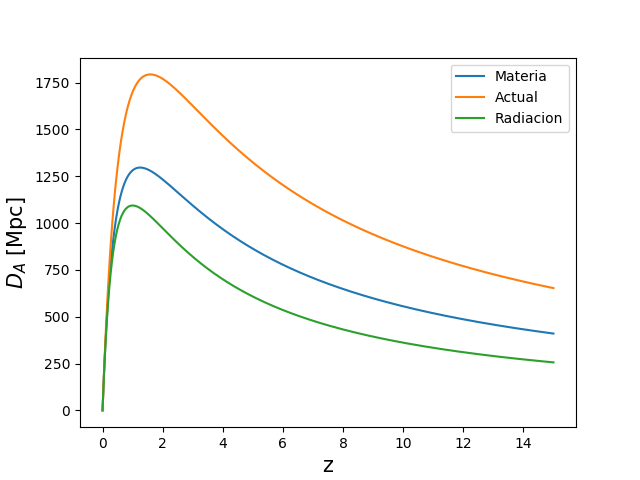
\includegraphics[scale=0.5]{DistanDiamAngular.png}
							\caption{Distancia diámetro angular $D_A$, en megaparsec, en función de $z$ para los universos dominados por Materia, dominado por Radiación, y para el universo actual según \cite{Plank}.}
							\label{Img:DisAng-All}
						\end{subfigure}%
						\begin{subfigure}{.5\textwidth}
							\centering
							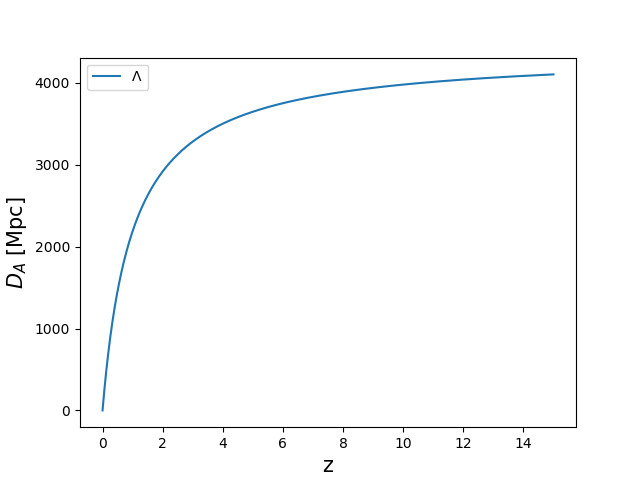
\includegraphics[scale=0.5]{DistanDiamAngular(EnrgOsc).png}
							\caption{Distancia diámetro angular $D_A$, en megaparsec, en función de $z$ para el universo dominado por energía oscura $\Lambda$.}
							\label{Img:DisAng-EngOsc}
						\end{subfigure}
						\caption{Distancia diámetro angular $D_A$, en megaparsec, en función de $z$ para los universos de estudios. En la Figura \ref{Img:DisAng-All} se muestran los universos dominados por Materia, dominado por Radiación, y el universo actual. A parte, en la Figura \ref{Img:DisAng-EngOsc}, se muestra el universo dominado por energía oscura $\Lambda$. Este universo se muestra separado del resto debido a que los valores de $D_A$ son varios ordenes de magnitud mayores, por lo que no se apreciaban los perfiles de los otros universos.}
						\label{Img:DisAng}
					\end{figure}

				En la Figura \ref{Img:DisLum} se muestran las distancias diámetro de luminosidad en función del \textit{redshift} $z$ para los cuatro universos de estudio.

					% Distancia Diematro Luminosidad
					\begin{figure}[H]
						\centering
						\begin{subfigure}{.5\textwidth}
							\centering
							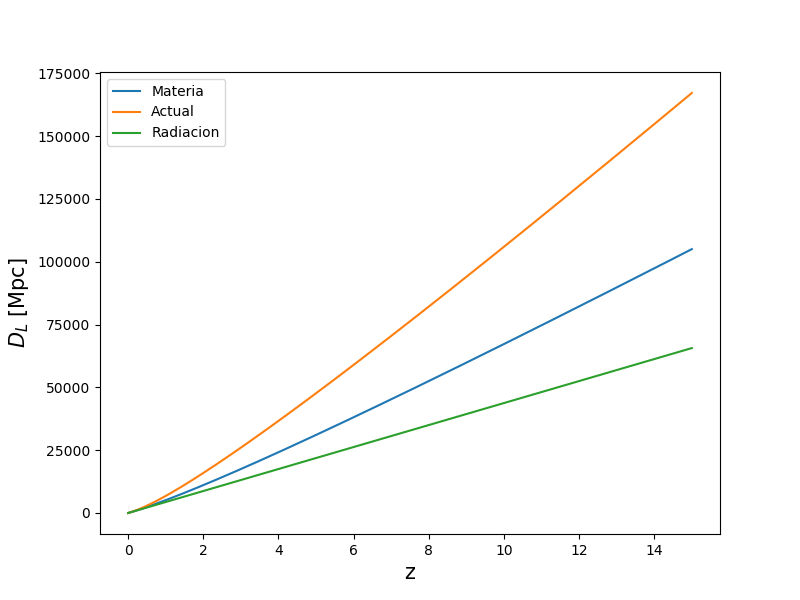
\includegraphics[scale=0.38]{DistanDiamLumino.png}
							\caption{Distancia diámetro de luminosidad $D_L$, en megaparsec, en función de $z$ para los universos dominados por Materia, dominado por Radiación, y para el universo actual según \cite{Plank}.}
							\label{Img:DisLum-All}
						\end{subfigure}%
						\begin{subfigure}{.5\textwidth}
							\centering
							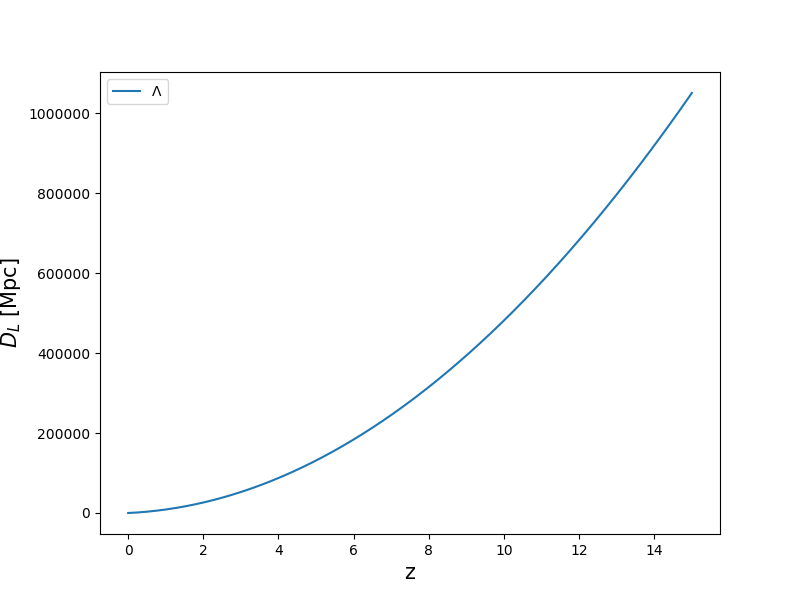
\includegraphics[scale=0.38]{DistanDiamLumino(EnrgOsc).png}
							\caption{Distancia diámetro de luminosidad $D_L$, en megaparsec, en función de $z$ para el universo dominado por energía oscura $\Lambda$.}
							\label{Img:DisLum-EngOsc}
						\end{subfigure}
						\caption{Distancia diámetro de luminosidad $D_L$, en megaparsec, en función de $z$ para los universos de estudios. En la Figura \ref{Img:DisLum-All} se muestran los universos dominados por Materia, dominado por Radiación, y el universo actual. A parte, en la Figura \ref{Img:DisLum-EngOsc}, se muestra el universo dominado por energía oscura $\Lambda$. Este universo se muestra separado del resto debido a que los valores de $D_L$ son varios ordenes de magnitud mayores, por lo que no se apreciaban los perfiles de los otros universos.}
						\label{Img:DisLum}
					\end{figure}

			\subsection{Factor de Escala \texorpdfstring{$a(t)$}{TEXT} y Parámetro de Hubble \texorpdfstring{$H(t)$}{TEXT}}
				\label{sec:a-H}

				Para obtener el factor de escala en función del tiempo ha sido necesario resolver la ecuación diferencial \ref{eq:EDOa} mediante métodos numéricos introduciendo la condición inicial $a_0 = 1$. En la Figura \ref{Img:FactorEscala} se muestran el Factor de escala $a(t)$ en función del tiempo para los cuatro universos de estudio.

					% Factor de Escala
					\begin{figure}[H]
						\centering
						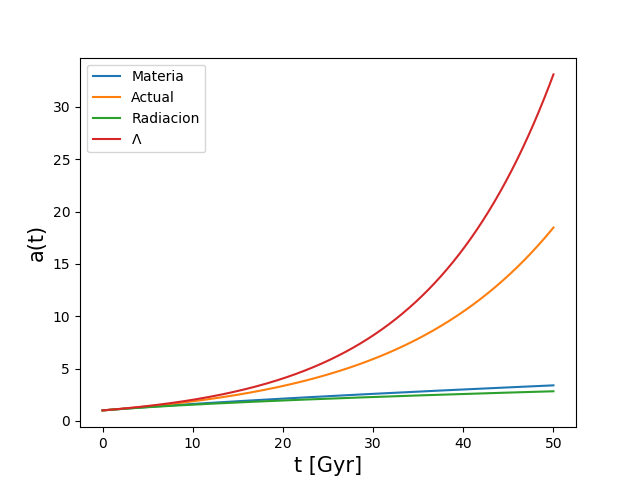
\includegraphics[scale=0.6]{factorEscala.png}
						\caption{\label{Img:FactorEscala}Factor de escala $a(t)$ en función del tiempo para los cuatro universos de estudio: Dominado por \textnormal{Materia}, dominado por \textnormal{Radiación}, dominado por energía oscura $\Lambda$ y con los parámetros del universo \textnormal{Actual} \cite{Plank}.}
					\end{figure}

				Una vez otenido el factor de escala en función del tiempo $a(t)$, la misma ecuación \ref{eq:EDOa} permite obtener el parámetro de Hubble $H(t)$. En la Figura \ref{Img:ParametroHbbl} se muestran el parámetro de Hubble $H(t)$ en función del tiempo para los cuatro universos de estudio.

					%H de t
					\begin{figure}[H]
						\centering
						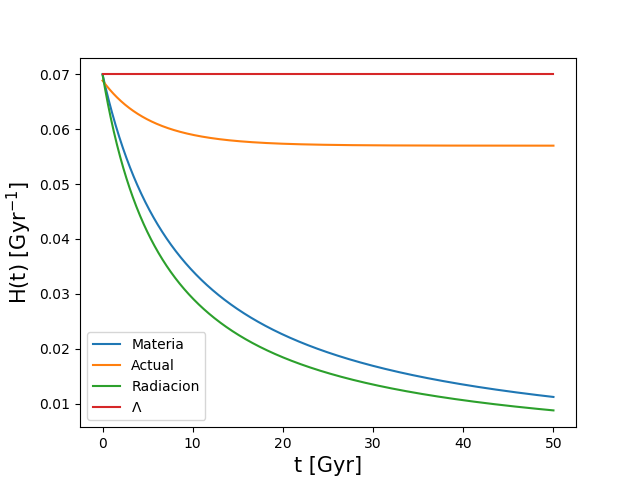
\includegraphics[scale=0.6]{H(t).png}
						\caption{\label{Img:ParametroHbbl}Parámetro de Hubble $H(t)$ en función del tiempo $t$ para los cuatro universos de estudio: Dominados por \textnormal{Materia}, dominado por \textnormal{Radiación}, dominado por energía oscura $\Lambda$ y con los parámetros del universo \textnormal{Actual} \cite{Plank}.}
					\end{figure}

			\subsection{Radio de Hubble y Horizonte de Partículas}
				\label{sec:RdHbll-HztPart}

				La ecuación \ref{eq:RadioHbbl} permite obtener el radio de Hubble a partir de los valores del parámetro de Hubble $H(t)$ de la sección \ref{sec:a-H}. En la Figura \ref{Img:RadHbbl} se muestran el radio de Hubble en función del tiempo para los cuatro universos de estudio.

					% Radio de Hubble
					\begin{figure}[H]
						\centering
						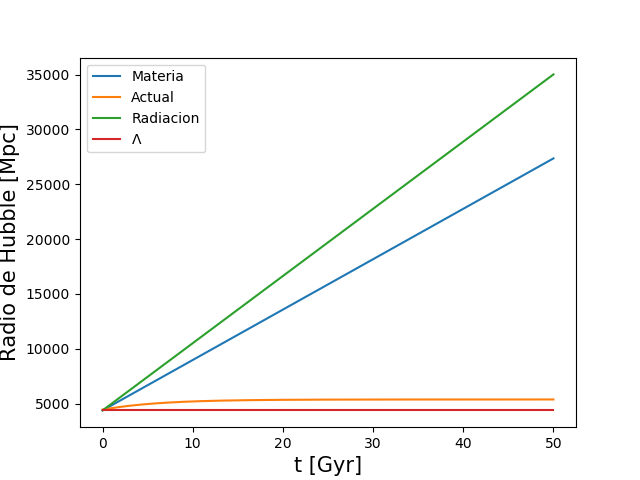
\includegraphics[scale=0.6]{radio_Hubble.png}
						\caption{\label{Img:RadHbbl}Radio de Hubble en función del tiempo $t$ para los cuatro universos de estudio: Dominados por \textnormal{Materia}, dominado por \textnormal{Radiación}, dominado por energía oscura $\Lambda$ y con los parámetros del universo \textnormal{Actual} \cite{Plank}.}
					\end{figure}

				De igual manera, la resolución del factor de escala $a(t)$ de la sección \ref{sec:a-H} permite obtener el horizonte de partículas a partir de la ecuación \ref{eq:HorizntPart}. En la Figura \ref{Img:HorztPart} se muestran el horizonte de partículas en función del tiempo para los cuatro universos de estudio.

					% Horizonte de Particulas
					\begin{figure}[H]
						\centering
						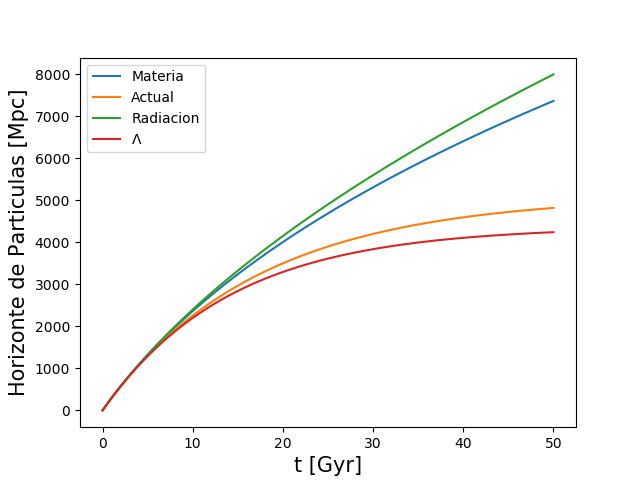
\includegraphics[scale=0.6]{horizonte_Particulas.png}
						\caption{\label{Img:HorztPart}Horizonte de partículas en función del tiempo $t$ para los cuatro universos de estudio: Dominados por \textnormal{Materia}, dominado por \textnormal{Radiación}, dominado por energía oscura $\Lambda$ y con los parámetros del universo \textnormal{Actual} \cite{Plank}.}
					\end{figure}
				
			\subsection{Edad del Universo}
				\label{sec:EddUniv}

				La ecuación \ref{eq:EddUniv} permite obtener la edad del universo en función del \textit{redshift} cosmológico $z$.En la Figura \ref{Img:EddUniv} se muestra la edad del universo en función del \textit{redshift} $z$ para los cuatro universos de estudio.

					% Edad del Universo
					\begin{figure}[H]
						\centering
						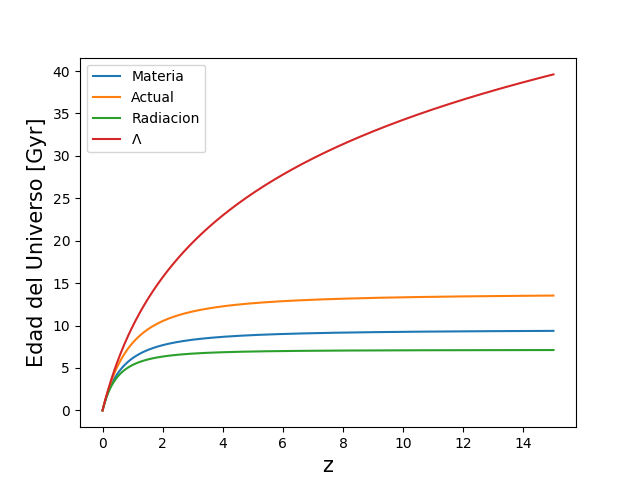
\includegraphics[scale=0.6]{edad_Universo.png}
						\caption{\label{Img:EddUniv}Edad del Universo en función del \textit{redshift} $z$ para los cuatro universos de estudio: Dominados por \textnormal{Materia}, dominado por \textnormal{Radiación}, dominado por energía oscura $\Lambda$ y con los parámetros del universo \textnormal{Actual} \cite{Plank}.}
					\end{figure}

				Cabe destacar que el \textit{redshift} cosmológico $z = 0$ corresponde al instante actual, y aumenta a medida que se va atrás en el tiempo, es decir, a medida que el \textit{redshift} aumenta la edad del universo también. Por lo tanto, para conocer la edad del universo se ha de integrar la ecuación \ref{eq:EddUniv} entre $z=0$ (instante actual) y $z=\infty$ (origen del universo).

					% RealEddUniv
					\begin{equation}
						t_{\textrm{Edad Universo}} = \frac{1}{H_0} \int_0^\infty \frac{\mathrm{d}z}{(1+z)E(z)} = 13.81 \textrm{ Gyr}
					\label{eq:EddUniv}
					\end{equation}

		\section{Conclusiones}

			Se han podido obtener las distancias diámetro angular $D_A$ y de luminosidad $D_L$, el factor de escala $a(t)$, el parámetro de Hubble $H(t)$, el horizonte de partículas, el radio de Hubble y la edad del universo para los cuatro universos de estudio mediante la resolución numérica de las ecuaciones de Friedmann a partir del código desarrollado en el lenguaje Python. Se ha realizado el estudio para tres universos dominados por Materia, Radiación y energía oscura $\Lambda$, y se ha añadido el estudio del universo Actual utilizando los parámetros de la misión Plank \cite{Plank}.

			Como caso general se ha obtenido que para el universo actual se han obtenido valores que se encuentran entre los obtenidos para Materia y Radiación, y el universo dominado por energía oscura, acercándose más a los valores del universo de energía oscura. Esto concuerda con el hecho de que el universo actual está dominado por la energía oscura con un $\Omega_\Lambda = 0.685$.

			En la sección \ref{sec:dL-dA} se han obtenido las distancias diámetro angular $D_A$ y de luminosidad $D_L$ en función del \textit{redshift}. Para estos valores ha sido necesario separar las gráficas del universo dominado por energía oscura del resto de universos debido a que éste toma valores de ordenes de magnitud mayor. Esto es debido a que para el universo dominado por la energía oscura la función $E(z)$ se convierte en una constante de valor la unidad. De esta forma, la coordenada radial depende linealmente del \textit{redshift}. Para este universo, en el caso de $D_A$ se obtiene una función logaritmica mientras que para $D_L$ se obtiene una función exponencial.

			Para el caso de los otros tres universos se observan perfiles similares en todos casos, siendo mayores los valores del universo actual y menores los valores del universo dominado por radiación. Esto es debido a la potencia de $(1+z)$ que multiplica a cada parámetro en $E(z)$. Para $D_A$ se observa un perfíl, común para los tres universos, dominado por un pico máximo entorno a $z\approx2$, disminuyendo los valores de $D_A$, a medida que aumenta $z$, de forma exponencial. Para el caso de $D_L$ se observa un aumento continuo con $z$, siendo mucho mayor este crecimiento para el universo Actual, acercandose al crecimiento exponencial del universo dominado por energía oscura $\Lambda$.

			Cabe destacar que según los datos de la calculadora \cite{CalculadorasI}, para \textit{redshift} $z=15$, los valores de $D_A$ y $D_L$ para los universos dominados por materia y el actual son los de la Tabla \ref{Tab:DA-DL}, que son similares a los obtenidos en la sección \ref{sec:dL-dA}.

				\begin{table}[H]
					\centering
					\begin{tabular}{ccc}
						\hline
						\centering
							Universo & $D_A$ [Mpc] & $D_L$ [Mpc] \\ \hline
							Materia & 416.9 & 106732.3 \\ 
							Actual & 652.7 & 167100.1 \\ \hline
					\end{tabular}
					\caption{\label{Tab:DA-DL}Distancia diámetro angular $D_A$ y de luminosidad $D_L$ para el universo actual y el dominado por materia para $z=15$ según \cite{CalculadorasI}}.
				\end{table}

			En la sección \ref{sec:a-H} se han obtenido el factor de escala $a(t)$ y el parámetro de Hubble en función del tiempo. Para estos casos se observa que los valores obtenidos para el universo actual se acercan mucho más a los del universo dominado por energía oscura, alejandose de los dominados por materia y radiación. En el caso del factor de escala $a(t)$, el aumento de $a(t)$ es claramente exponencial para el universo dominado por energía oscura y el universo actual. Esto concuerda con la teoría vista en clase donde se vió que para el universo \textit{de Sitter} en el que domina la energía oscura, que equivale al universo $\Lambda$ estudiado, el factor de escala evoluciona como $e^{H_0t}$. De forma muy similar evoluciona el universo Actual dominado por energía oscura. El hecho de que tome valores menores es debido a la contribución de materia que existe. Esto es debido a la gran contribución de la energía oscura a la expansión del universo.

			Por el contrario, para los universo dominados por materia y radiación la evolución del factor de escala $a(t)$ no es exponencial, llegando a parecer casi lineal debido a la comparación con los universos con mayor contribución de energía oscura. No obstante, este crecimiento puede asemejarse al visto en clase, que para el caso del universo dominado por radiación es $a(t) \propto t^{1/2}$ y para el caso del universo de \textit{Einstein-de Sitter} dominado por materia $a(t) \propto t^{2/3}$.

			Para el parámetro de Hubble se ha dividido la derivada del factor de escala entre el propio factor de escala. De esta manera se ha obtenido un comportamiento constante del $H(t)$ para el universo dominado por energía oscura $\Lambda$ con un valor de $H(t) \approx 0.7$. Para el resto de universos se poduce una clara dismunución de $H(t)$ para valores pequeños de $t$, que para el caso de los universos dominados por Materia o por radiación continua disminuyendo de forma exponencial. No obstante, para el caso del universo actual con gran contribución de energía oscura, esta disminución inicial es algo menor, cesando para valores $t \approx 20$ Gyr y evolucionando de manera constante paralelo a los valores del universo $\Lambda$.

			En la sección \ref{sec:RdHbll-HztPart} se han obtenido valores para el radio de Hubble y el horizonte de partículas en función del tiempo $t$. Nuevamente, para ambos valores se puede diferenciar los comportamientos de los universos dominados por Materia y Radiación del comportamiento de los universos con presencia de energía oscura (Actual y $\lambda$). En este caso los valores obtenidos para los universos con presencia de energía oscura son mucho menores que los obtenidos para los universos dominados por Materia o por Radiación, llegando a ser 2 o 7 veces mayores. Para el caso del radio de Hubble, los valores se han obtenido a partir de la inversa del parámetro de Hubble según la ecuación \ref{eq:RadioHbbl}, por lo que cabe esperar que su comportamiento equivalga a la inversa del obtenido en la sección \ref{sec:a-H} para el parámetro de Hubble. Efectivamente, se puede observar como para el unvereso completamente dominado por energía oscura el radio de Hubble se mantiene constante. También se observa como para el universo actual el radio de Hubble aumenta al principio pero se estabiliza rápidamente manteniendose constante y paralelo a los valores de la energía oscura. No obstante, para el caso de los universos dominados por Materia o por Radiación el radio de Hubble aumenta de forma constante con el tiempo, siendo mayor para el universo dominado por radiación. Esto parece consistente con el hecho de que este radio hace referencia a la distancia a la cuál los objetos se alejan a una velocidad de recesión igual a la velocidad de la luz.

			Por otro lado, el horizonte de partículas ha sido obtenido a partir de la integral de la inversa del factor de escala a partir de la ecuación \ref{eq:HorizntPart}. Los cuatro universos describen un perfil similar en el que se puede observar un aumento del horizonte de partículas de forma logaritmica disminuyendo su crecimiento con el tiempo. No obstante, mientras que para los universos Materia y Radiación dicho aumento no parece cesar y hace pensar que va a seguir aumentando con el tiempo, para los universos con presencia de energía oscura sí se aprecia una estabilización que hacen pensar que el horizonte de partículas podría tomar un valor máximo o constante.

			Por último, en la sección \ref{sec:EddUniv} se ha obtenido la edad del universo en función del \textit{redshift} a partir de la ecuación \ref{eq:EddUniv}. En este caso, el comportamiento de la edad del universo en función de $z$ para el universo Actual se parece más al comportamiento de los universos Materia y Radiación, con ausencia de energía oscura. Para el universo dominado por energía oscura se observa un comportamiento logaritmico con un gran aumento que parece tomar el valor infinito para un redshift infinito, que como, hemos visto en la introducción, equivaldría al orígen del universo al tomar el convenio \textit{look-back time}. Esto quiere decir, que en el caso de un universo dominado por energía oscura no se podría hablar de un origen del universo, pues se encontraría en un tiempo infinito. por el contrario, para los otros tres universos el comportamiento legaritmico es mucho menor y sí parece estabilizarse hacia un valor constante. Esto hace pensar que para estos tres tipos de universo sí puede existir un origen del universo, situado en un tiempo determinado. Este tiempo en el que se sitúa el origen del universo, edad del universo, es mucho menor para el universo dominado por la radiación, por lo que se trataría de un universo mucho más joven. El universo dominado por Materia tiene una edad del universo mayor que el universo dominado por radiación, pero menor que el universo Actual con los parámetros actuales \cite{Plank}. Para este universo en concreto se ha determinado la edad del universo tomando ésto como el tiempo para un \textit{redshift} infinito $z = \infty$. De esta forma se ha obtenido una edad del universo actual de $t = 13.81$ Gyr. Dicho valor es perfectamente compatible con el valor que en la actualidad se considera como la edad del universo que es de $t = 13.8$ Gyr \cite{NasaEdadUniv}.

			No obstante, cabe destacar que en este estudio se ha trabajado en todo momento con universos planos, considerando la curvatura nula $\Omega_K = 0$. Esto se ha realizado por semejanza con los valores actuales de la curvatura del universo, pero el estudio de estos parámetros puede dar información de interes para los casos con curvatura tanto positiva como negativa.
	%\end{multisecols}

%----------------------------------------------------------------------------
%     APPENDIX
%----------------------------------------------------------------------------

\newpage

	    \appendix

	    	\section{Descripción del \textit{Software} desarrollado}
	    		\label{appen:N1}

	    		Para la realización de la Calculadora Cosmológica se ha desarrollado un programa escrito en el lenguaje Python (\textit{Python2.7}) para la resolución numérica de las ecuaciones y la representación de los datos. El código del programa se ha dividido en tres Scripts: \texttt{main.py}, \texttt{ representarGraf.py} y \texttt{CalcCosmlgc.py}.

	    		Todos los cálculos realizados para la calculadora cosmológica se han realizado en el script \texttt{CalcCosmlgc.py}. En dicho script se define una clase objeto \texttt{CalcCosmologica()} al cuál se le pasan como atributos los parámetros de densidad $\Omega_X$ y la constante de Hubble $H_0$, definiendo así el tipo de universo del que se trata. Los métodos de esta clase son los necesarios para calcular todos los valores que se piden. En el script \texttt{ representarGraf.py} se define otra clase a la que se le pasa un diccionario de python con los universos que se quieren estudiar, con sus nombres, y los valores del redshift $z$ y del tiempo $t$ en los que se quiere realizar el estudio,  y se representan los diferentes valores en gráficas. Por último, el script principal \texttt{main.py} permite crear los arrays de $z$ y $t$, así como el diccionario con los diferentes universos, y llamar a los métodos del script \texttt{ representarGraf.py} para obtener las gráficas. El script \texttt{ representarGraf.py} guarda las gráficas en una carpeta \textit{Graficas/}.

	    		En el desarrollo del código se han utilizado diferentes paquetes de librerías disponibles para Python tales como: \textit{numpy, scipy} y \textit{matplotlib}. De estos paquetes caben destacar los métodos utilizados para la resolución de las integrales definidas y de la ecuación diferencial resuelta para la obtención de $a(t)$.

	    		Para la resolución numérica de las integrales definidas se ha utilizado la función \texttt{integrate.quad()} del paquete SciPy. Esta función está basada en la librería QUADPACK  de Fortran que realiza la integral utilizando el método de cuadratura numérica.

				\begin{lstlisting}[style=python]
import scipy.integrate as integ

integral = np.zeros(len(z))
for i in range(len(z)):
    integral[i], err = integ.quad(lambda x:1/self.E(x), 0, z[i])
				\end{lstlisting}

	    		Para la obtención de $a(t)$ ha sido necesario resolver de forma numérica la ecuación diferencial \ref{eq:EDOa}. Para ello se ha utilizado la función \texttt{integrate.ode()} del paquete SciPy. Este paquete permite resolver la ecuación diferencial $y'(t) = f(y(t), t)$ a partir de métodos integradores numéricos, permitiendo escoger que método utilizar. El método utilizado ha sido el "dopri5", el cuál utiliza el método runge-kutta de orden 4(5). Además, también permite determinar unas condiciones iniciales para la ecuación diferencial. Para el caso del factor de escala la condición inicial impuesta es $a(t=0) = 1$.

	    		\begin{lstlisting}[style=python]
import scipy.integrate as integ

r = integ.ode(aPunto).set_integrator("dopri5")
r.set_initial_value(1, 0) # a(t=0) = 1
for i in range(1, len(t)):
	a[i, :] = r.integrate(t[i])
				\end{lstlisting}

				Cabe destacar que para el caso del horizonte de partículas ha sido necesario realizar la integral definida de la inversa de la función $a(t)$, por lo que dentro de la función \texttt{integrate.quad()} se ha tenido que llamar a la función que resuelve la EDO. Esto ha supuesto que en ciertos momentos se haya tenido que llamar al método "dopri5'' con pocos valores de $t$ para su resolución, y añadir a los valores de $t$ dados, el valor de la condición inicial $t = 0$.

			\section{Ejecución del Programa}

				Antes de ejecutar el programa es importante asegurarse de que existe una carpeta llamada \textit{Graficas/} en el directorio desde el que se vaya a ejecutar el programa, de tal forma que el script \texttt{ representarGraf.py} pueda guardar las gráficas en él. En caso contrario habría que cambiar dicho directorio en el script \texttt{ representarGraf.py}.

				Puesto que se trata de un programa escrito en python, para su ejecución tan solo hay que escribir el siguiente comando en la terminal.

				\begin{center}
					\begin{minipage}[c]{200pt}
						\begin{listing}[style=consola, numbers=none]
$ python main.py
						\end{listing}
					\end{minipage}
				\end{center}

				En caso de querer variar tanto los valores de $z$ y $t$ de estudio como los tipos de universo, se podrá realizar modificando dichos valores directamente en el script \texttt{main.py}, teniendo en cuenta que $H_0$ ha de ir en $Gyr^{-1}$.
%----------------------------------------------------------------------------
%     BIBLIOGRAPHY
%----------------------------------------------------------------------------

	\nocite{Calculadoras}
	\nocite{codigo}

	\bibliographystyle{unsrt}
	\bibliography{biblio}

\end{document}


%----------------------------------------------------------------------------
%            TEMPLATES
%----------------------------------------------------------------------------

%----------------------------------------------------------------------------
%            how to insert an image
%----------------------------------------------------------------------------

%	\begin{figure}[H]
%		\centering
%		\includegraphics[scale= ]{nombre de la imagen.jpg}
%		\caption{\label{Img:widgets}el pie de pagina que le quieras 	poner a la imagen}
%	\end{figure}
 
%----------------------------------------------------------------------------
%            how to insert a table
%----------------------------------------------------------------------------

%	\begin{table}[H]
%		\centering
%		\begin{tabular}{|c|c|c|c|}
%			\hline
%			\centering
%				Altura(h) & Distancia (d) & Elaboracion (e) & Longitud (l) \\
%				($\pm0.5$ mm) & ($\pm0.5$ mm) & ($\pm0.5$ mm) & ($\pm0.5$ mm) \\ \hline
%				 &  &  &  \\ \hline
%				 &  &  &  \\ \hline
%				 &  &  &  \\ \hline
%				 &  &  &  \\ \hline
%				 &  &  &  \\ \hline
%		         &  &  &  \\ \hline
%		\end{tabular}
%		\caption{\label{Tab:widgets}pie de pagina que le quieras poner}
%	\end{table}

%----------------------------------------------------------------------------
%             How to remove the label in equactions
%----------------------------------------------------------------------------

%	\begin{equation*}
%		
%	\end{equation*}

%----------------------------------------------------------------------------
%              How to set bibliography
%----------------------------------------------------------------------------

%\bibliographystyle{unsrt}
%\bibliography{biblio}
%
%Then you have to set a .bib document such as the next template
%
%	@book{nickname,
%	author = {},
%	title = {},
%	edition = {},
%	year = {},
%	volume = {},
%	ISBN = {}
%	}
%
%	@ARTICLE{nickname,
%	author = {},
%	title = {},
%	year = {},
%	volume = {},
%	}


%----------------------------------------------------------------------------
%              END
%----------------------------------------------------------------------------
